\chapter{MANTA Flow platform}

Before we get into the details of data lineage analysis service for embedded code, let us first introduce and describe MANTA Flow platform. It is the platform that the service is integrated with and influences many of the design and implementation decisions. It also provides a couple of solution examples for problems we might face that we will use for inspiration.

%---------------------
% SECTION
%---------------------
\section{Data lineage}

Data lineage refers to the tracking of data from its source to its destination and all the transformations and processes it undergoes along the way. It is the complete end-to-end history of data flow, including its origins, where it has been, and how it has been altered.
\par
The purpose of data lineage is to ensure that data is accurate, trustworthy, and complies with regulatory and compliance requirements. It provides transparency into data transformations, allowing organizations to understand how data has been changed. Data lineage is also used to identify and resolve data quality issues and to support data governance and management initiatives. From an engineering point of view, it can help developers to integrate data from multiple sources more efficiently and ensure that data is accurately transferred and transformed throughout the system. Overall, data lineage plays a crucial role in improving the reliability, efficiency, and effectiveness of data-driven decision-making.
\par
Data lineage can be obtained by hand from teams of analysts that map data environments or, more recently, using one of the automated systems that are being developed. Manual data lineage analysis is time- and labor-intensive, so developing automated solutions can provide more up-to-date results and decrease costs.

%---------------------
% SECTION
%---------------------
\section{MANTA Flow overview}

MANTA Flow is an automated data lineage platform that scans data environments to build and visualize a graph of all data flows within it. This graph enables its users to get better visibility and control of their data pipeline.
\par
Each data environment consists of a different set of databases, tools and other technologies. In order to build a data lineage graph for the entire environment, MANTA Flow uses a wide range of proprietary scanners. Each scanner can analyze data lineage for a single technology (we will use the term \textit{technology} to uniformly describe databases, ETL/reporting tools and programming languages supported by MANTA platform). These partial graphs are then combined in metadata repository to provide the output for the entire environment.
\par
TODO: describe scenarios, CLI, why metadata is used.

%---------------------
% SECTION
%---------------------
\section{Scanners}

A scanner provides data lineage for a particular technology. This process consists of multiple steps and varies for each technology based on its type. The data lineage is created from metadata and scripts, so the execution of a scanner is split into two general scenarios: metadata extraction and dataflow analysis.

\subsection{Metadata extraction}

Metadata extraction scenario usually, as the name suggests, extracts metadata required for the dataflow analysis. Other artifacts could be extracted, too, such as scripts of any kind, configuration etc. The purpose of this scenario is to gather all resources needed for dataflow analysis and store them locally so that the analysis can be executed in \textit{offline} mode, that is, without requiring an active connection to any other system.
\par
There are multiple reasons why metadata extraction is a standalone scenario. Here is a list of some that are relevant in the context of this thesis:
\begin{itemize}
    \item The analyzed systems are not directly accessible from \textit{MANTA Flow} server. \textit{MANTA Flow Agent} is a component that can be configured to perform the extraction on a remote device which has network access to these systems and then securely transfer the extracted artifacts back to \textit{MANTA Flow} server. 
    \item When errors occur during extraction, the user can fix them before executing dataflow analysis.
    \item In some cases, the user may want or have to provide additional input, e.g., configuration not provided via any available API, additional mapping information etc.
\end{itemize}

\subsection{Dataflow analysis}

Dataflow analysis discovers dataflows in target systems using the extracted inputs. There are multiple steps in this process and the specifics vary between different technologies.
\par
One of the steps is \textit{DDL dataflow scenario}. This scenario processes DDL (Data Definition Language) constructs 
- DDL dataflwo scenario
- Dictionary mapping scenario - links to query service
- Dataflow scenario - script analysis
- Graph contains nodes which are either transformations or data sources, explain graph in an earlier point


% Description of query service, how it works, similarities to what we are trying to achieve.
%- it has a common interface
%- usually used when the connection details are not entirely known
%- could also be that nothing is known
%- can deduce
%- only resolves queries for which it constructs nodes
%---------------------
% SECTION
%---------------------
\section{Dataflow Query Service}

Dataflow Query Service is a component that helps with processing of embedded SQL queries. It works by selecting the appropriate embedded language scanner for the provided input, executing dataflow analysis and merging the resulting sub-graph into the graph of the original data technology scanner.
\par
Often, data technologies such as reporting or ETL tools use SQL to define data sources. Such SQL queries are used to query data from a connected database without the need to create a dedicated table or a view. Since Manta Flow contains scanners for most common database systems, they are already able to process these queries. Dataflow Query Service groups these scanners in a unified service that can be used by other data technologies.
\par
One of the main benefits of this service is that it uses metadata extracted by each scanner, therefore it has access to extracted database schemas, which allows it to resolve exact columns for queries such as \texttt{SELECT * FROM TABLE\_A}. It is also useful in situations when details about the target systems are unknown or unresolved, the service has the ability to deduce columns from available information and to choose the appropriate scanner from the provided connection details.

\subsubsection{Overview}
In general, there are three pieces of information needed to analyze an SQL query:
\begin{itemize}
    \item Connection data - connection type, connection string, server hostname (at least connection string or server name is needed).
    \item Default data - default database, default schema, connecting user (as applicable) in case connection data is not available or not recognized.
    \item Query or embedded script text.
\end{itemize}
If the data technology scanner has all of the above information, it constructs a \texttt{Connection} object directly, otherwise it is expected to perform connection mapping by retrieving the required data from manual configuration. Connection and query text are inputs for Dataflow Query Service. Next, dictionary mapping is performed, that is, an appropriate target scanner and a persisted data dictionary is selected based on \texttt{Connection} data. The selected scanner is invoked with query text, data dictionary and defaults, which provides the result in form of a \texttt{DataflowQueryResult}. The data technology then uses this result to connect the resulting lineage to the relevant nodes in the host script and to merge the result into the main graph.

\subsubsection{External connections}
One of the main purposes of \texttt{DataflowQueryResult} is to perform connection to external nodes. The purpose of embedded queries is to provide data for further processing, therefore we would like to connect the nodes of the query objects with other nodes in the lineage, e.g., connect database columns with data fields in a report. These connection points are unknown to the query scanner and the host scanner doesn't understand the query in advance, so the result graph contains extra nodes called \textit{pin} nodes.
\par
Pin nodes represent an input to a node representing query parameter or an output from a query resultset column. After the query is analyzed and its graph is created, the service adds these pin nodes and connects them with appropriate edges to the result nodes. Then, the host scanner might provide a mapping from pin nodes to nodes in the host graph. The service creates new edges from pin nodes to host graph nodes (and vice versa, depending on the direction) based on the provided mapping and then contracts the pin nodes, thus effectively connecting the resultset column node or a parameter node with the host graph node. Should any pin node remain unmatched, it is filtered out in filtering task later in the scenario.

\subsubsection{Architecture}
%%% copied from Confluence, can I somehow quote this?
\begin{figure}[ht]\centering
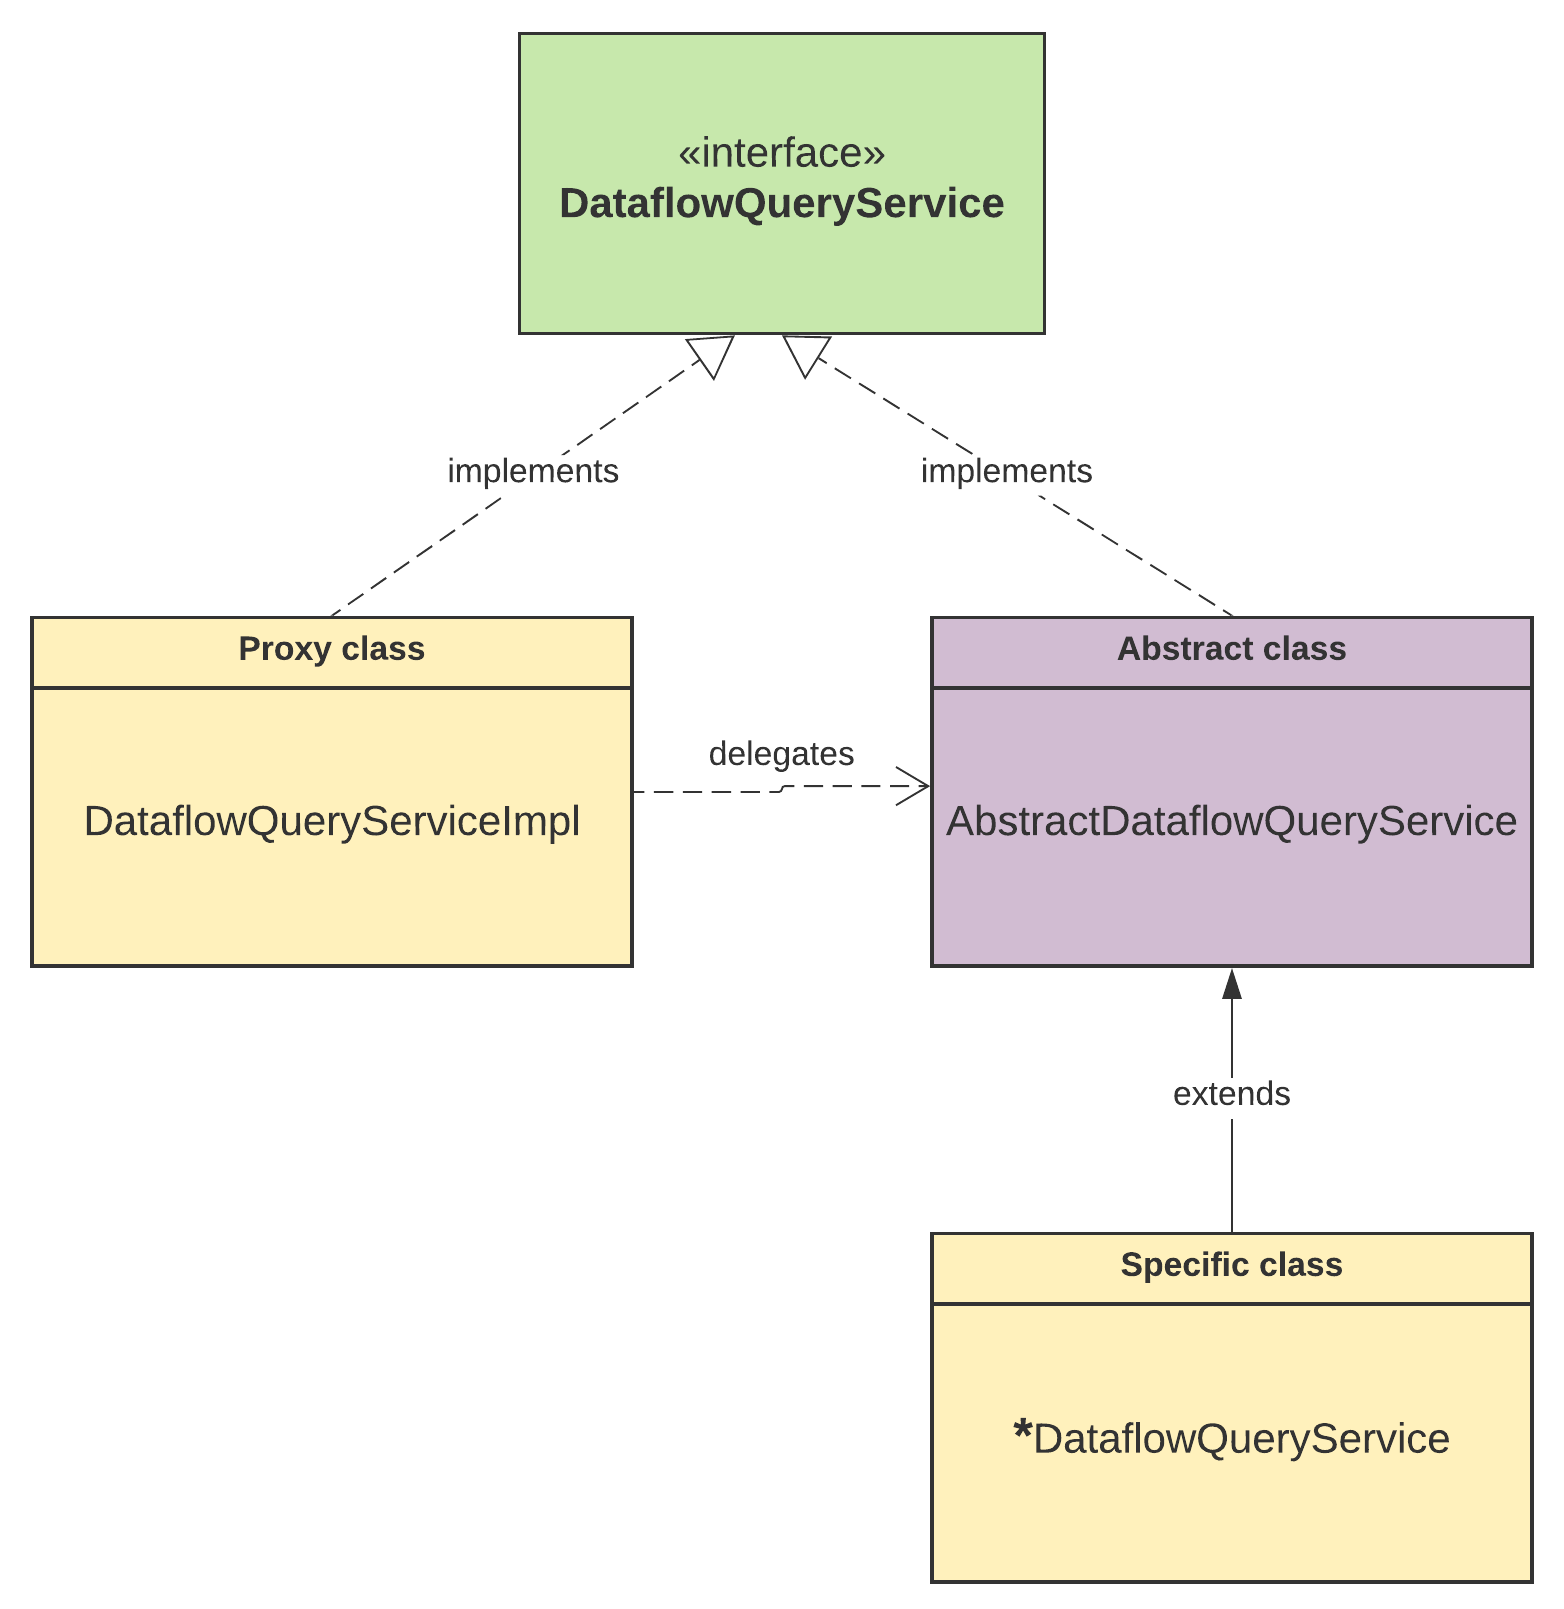
\includegraphics[width=1.0\textwidth]{img/cls.png}
\caption{A simplified class diagram of Dataflow Query Service}
\label{fig01:QS}
\end{figure}  


\texttt{DataflowQueryService} is a common interface that provides methods for client scanners for analyzing SQL queries or creating hierarchical database structures. This interface is implemented by:
\begin{itemize}
    \item Individual database query services that contain logic for providing data flows or hierarchical database structures.
    \item Proxy class called \texttt{DataflowQueryServiceImpl} that wraps all other individual query services. It is a classic implementation of a proxy class that chooses a specific query service based on information provided in the connection from the caller and delegates the operation.    
\end{itemize}

A simplified class diagram is depicted in figure~\ref{fig01:QS}.





%---------------------
% SECTION
%---------------------
\section{Language scanners}
Description of language scanners, their composition, how they work
- no DDL/dictionaries, only scripts
- extraction is just a preparation of the input
- analysis uses worklist algorithm, intermediate dataflow generator, common output
- differences with database scanners
- 

%---------------------
% SECTION
%---------------------
\section{Python scanner}